\documentclass{beamer}


\usepackage{amssymb}
\usepackage{amsmath}
\usepackage{amsfonts}

\usepackage{fontspec}
\usepackage{polyglossia}

\usepackage{graphicx}
\usepackage{color}
\usepackage{url}
\usepackage{textpos}
\usepackage{xspace}
\usepackage{array}


\graphicspath{{./fig/}}


\title{Morphological Segmentation for Machine Translation\\
\scriptsize{in Elx, 2014}}
\author{Tommi A Pirinen \scriptsize \guilsinglleft{}tommi.pirinen@computing.dcu.ie\guilsinglright{}}
\institute{DCU, CNGL\\Abumatran}
\date{\today}

\begin{document}

\selectlanguage{english}

\maketitle

\section{Introduction}

\begin{frame}
    \frametitle{About myself}
    \begin{itemize}
        \item BSc in CS from U Joensuu (now UEF.fi) 2004, 
            MA in Comp Ling from U Helsinki 2008
            and PhD in Comp Ling from U Helsinki 2014
        \item CL projects such as:
            open source morphology of Finnish,
            giellatekno comp ling repo,
            HFST,
            apertium (fin-{eng,swe,hun,hbs,ces,gle,rus} etc.)
        \item Other FLOSS projects:
            Gentoo Linux,
            Finnish localisation,
            probably more
    \end{itemize}
\end{frame}

\begin{frame}
    \frametitle{Background: Morphological complexity}
    \begin{itemize}
        \item debated, hot topic in linguistics
        \item for MT measuring is relatively simple:
        \item number of unique tokens / oov tokens per dataset, etc.
        \item e.g., most English nouns have \textasciitilde 4 forms (plural + possessives)
            Serbo-Croatian at least 14 (cases, plurals), 
            Finnish at least 5,271 (cases, plurals, possessives, clitics,'
            allomorphs)
        \item with compounding and derivation vocabulary is practically endless
        \item So, amount of data for statistical models might need to be more

    \end{itemize}
\end{frame}

\begin{frame}
    \frametitle{Motivation / Use cases}
    i.e., what is it good for:
    \begin{itemize}
        \item Morphology-aware terminology management in localisation
            applications
        \item there's practically very little localisation software that
            handles morphology with terms, names etc. well
        \item e.g., software localisation I've seen so far doesn't quite allow
            for morphology at all (gettext etc.)
        \item e.g., translation memories will fuzzy match copy the most common
            forms forcing translators to post editorially inflect all terms
    \end{itemize}
\end{frame}

\begin{frame}
    \frametitle{Morphological segmentation}
    \begin{itemize}
        \item For MT: ideally break wordform down to morphs that would translate
            to words in the other language
        \item e.g. talo : talo/ssa : talo\_i/hin : puu/talo etc. for house : in house : to house\_s : wooden house (Finnish and English share plural as suffix)
        \item segmentation can be ambiguous, e.g. katos/ta \textasciitilde{}
            kato/sta (between katto and katos)
        \item with rulebased morphology we can select these rather easily
        \item statistical approach such as Morfessor uses minimum description
            length with corpora learning to segment the likely morphs to
            minimize number of unique morphs in whole data; may need tuning
            and data selection
        \item N.B. alternative to morphological segmentation would be to use
            factored models with morphological analyses and lemmatization or
            stemming
    \end{itemize}
\end{frame}

\begin{frame}
    \frametitle{Segmentations in Translation}
    When semantic case suffixes are used prototypically they align 1:1 English.
    When semantic cases are e.g. object cases of the verb in a construction
    they can be more complex though.
    \includegraphics[width=\textwidth]{alignments}
\end{frame}

\begin{frame}
    \frametitle{Europarl statistics for English, Finnish and two segmentations}
%    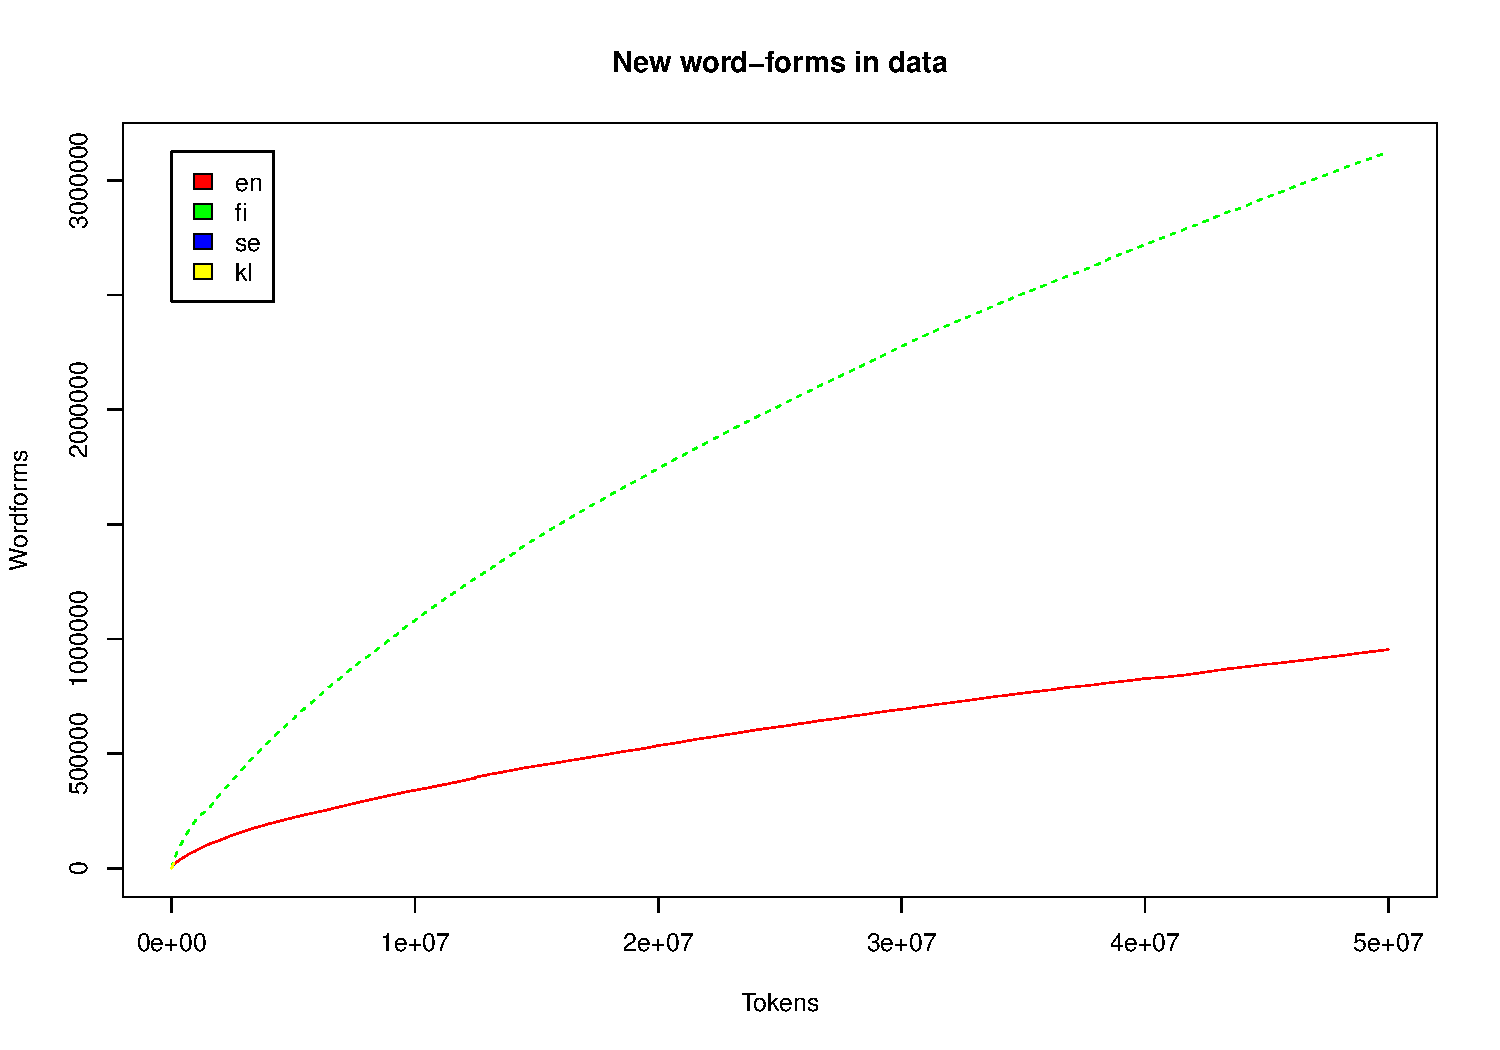
\includegraphics[width=\textwidth]{formspertokens}
\end{frame}

\section{Implementation}

\begin{frame}
    \frametitle{Implementation: Baseline Moses}
    This is starting point for all my experiments
    \begin{itemize}
        \item as per \url{http://www.statmt.org/moses/?n=Moses.Baseline}
        \item Split corpus, tokenize, truecase, clean
        \item train Language models
        \item align, train translation model
        \item tuning
        \item test set is tokenised, truecased, translated, and compared
    \end{itemize}
\end{frame}

\begin{frame}
    \frametitle{Morphological segmentations}
Translating \emph{from} morphologically complex language (e.g., Fin $\rightarrow$ Eng)
    \begin{itemize}
        \item training corpus is segmented on source language side (e.g., Fin)
            before training translation model
        \item test set needs to be segmented before translating
        \item morph lattices can be used instead of 1-best segmentation
    \end{itemize}
    Translating \emph{into} morphologically complex language (e.g., Eng $\rightarrow$ Fin)
    \begin{itemize}
        \item training corpus is segmented on target language side (e.g., Fin)
            before training language and translation models 
        \item translation need to be joined before evaluating
        \item what to do with stray segments and illegal combinations
    \end{itemize}
\end{frame}

\begin{frame}
    \frametitle{Morph lattices}
    Ambiguous segmentations and statistical n-best segmentations can be fed to
    moses as if they were word lattices:
    \only<1>{
    \includegraphics[width=\textwidth]{lattice}\\
    (from morfessor's 2-best segmentation; morphologically correct:
    ``Kaikki ihmise/t synty/vät vapa/i/na ja tasa/vertais/i/na arvo/lta/an ja
    oikeuks/i/lta/an'')
}
\only<2>{
    \includegraphics[trim=400 0 600 0,clip,width=\textwidth]{lattice}\\
}
\end{frame}

\begin{frame}
    \frametitle{Morphological segmentations and statistics}
    \begin{itemize}
        \item Rule-based segmentation needs either analyser trained with
            good statistics or segmentation trained with good segmentations
        \item Some morfessor algorithms can be trained with gold data
        \item There's not much pre-segmented data available
        \item currently what I did is use automatic segmentations of different
            sources to give some statistics (or weights of WFSA analyser if
            available)
    \end{itemize}
\end{frame}

\begin{frame}
    \frametitle{The Experiments}
    Writing comparison of results with different parameters:
    \begin{itemize}
        \item Different segmentation algorithms: Rule-based (morphs,
            words), Morfessor (2.0, categories map, ml)
        \item Different size of training data for segmenters: europarl
            partitions (full, half, quarter, eighth)
        \item Different size of training data for translation model:
            same europarl partitions
        \item Joining algorithms
    \end{itemize}
\end{frame}

\begin{frame}
    \frametitle{The Results}
    \begin{tiny}
    WIP as of \today: \\
    English to Finnish\\
        \begin{tabular}{|l|r|r||r|r|}
            \hline
            Score: & \bf BLEU & \bf TER  & \bf BLEU  & \bf TER   \\
            Model  & (in dom) & (in dom) & (out dom) & (out dom) \\ 
            \hline
            \bf Apertium Baseline      & 0.03 & & 0.01 & 0.96 \\
            \hline
            \bf Moses Baseline         & 0.15 & & 0.18 & 0.71 \\
            \hline
            \bf Moses 1-Best Compounds (FSA) & 0.15 & & 0.17 & 0.70 \\
            \hline
            \bf Moses 1-Best Morphs (FSA + Morfessor) & 0.14 & & 0.10 & 0.74 \\
            \hline
            \bf Moses 1-Best Morphs (Morfessor) & & & &  \\
            \hline
        \end{tabular}
    \end{tiny}
\end{frame}

\begin{frame}
    \frametitle{The Results}
    \begin{tiny}
    WIP as of \today: \\
    Finnish to English\\
        \begin{tabular}{|l|r|r||r|r|}
            \hline
            Score: & \bf BLEU & \bf TER  & \bf BLEU  & \bf TER   \\
            Model  & (in dom) & (in dom) & (out dom) & (out dom) \\ 
            \hline
            \bf Apertium Baseline      & & & &  \\
            \hline
            \bf Moses Baseline         & & & &  \\
            \hline
            \bf Moses 1-Best Compounds (FSA) & & & &  \\
            \hline
            \bf Moses 1-Best Morphs (FSA + Morfessor) & & & & \\
            \hline
            \bf Moses 1-Best Morphs (Morfessor) & & & &  \\
            \hline
        \end{tabular}
    \end{tiny}
\end{frame}
\begin{frame}
    \frametitle{Future World}
    \begin{itemize}
        \item Include more languages in tests: South Slavic, 
        \item Limit segmentation to rare words instead of all
        \item Error analysis should reveal some interesting things
        \item Segmentation gold standards
        \item \ldots (suggestions welcome)
    \end{itemize}
\end{frame}

\begin{frame}
    \frametitle{URLs and references}
    \begin{itemize}
        \item \url{Tommi.Pirinen@computing.dcu.ie}
        \item \url{http://www.computing.dcu.ie/~tpirinen/} 
        \item \url{http://www.github.com/flammie/purplemonkeydishwasher/}
        \item SVN at redmine repo mt-development
    \end{itemize}
\end{frame}

\bibliography{morph-segments}

\end{document}
% vim: set spell:
